% Hidden and exposed terminal problems in Wi-Fi
% Author: Philip Withnall
\documentclass{article}
\usepackage{tikz}
\usetikzlibrary{decorations.pathreplacing} % for expanding waves

% Style for radio transmission paths.
\tikzstyle{transmission}=[decorate, decoration={expanding waves, angle=7,
                          segment length=2}]

% Path definition for a base station. Parameters
%  1. Node name.
%  2. Node label.
%  3. Path graphic options.
\newcommand{\basestation}[3]{%
	\path[draw, thick, #3] (0, 0) node(#1){#2}
			(0*120+90:0.5cm) --
			(1*120+90:0.5cm) --
			(2*120+90:0.5cm) -- cycle
}

\begin{document}
\begin{center}
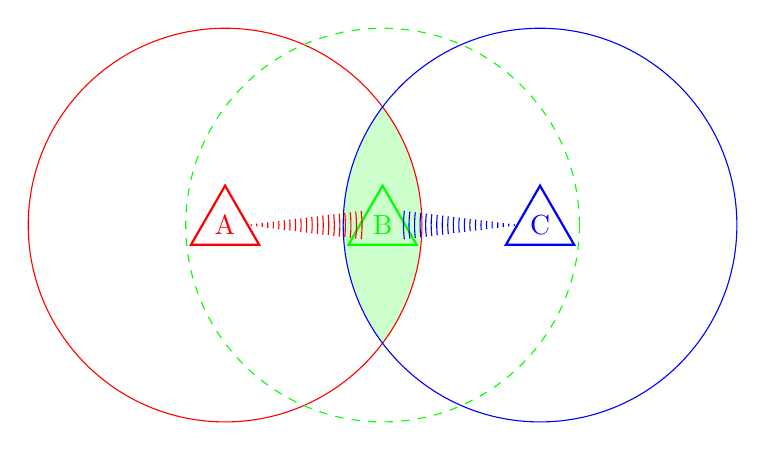
\begin{tikzpicture}
	% Shade the intersection where signals collide.
	\begin{scope}
		\clip (-2, 0) circle [radius=2.5];
		\fill[fill=green!20] (2, 0) circle [radius=2.5];
	\end{scope}

	% Signal radii.
	\draw[red] (-2, 0) circle [radius=2.5]; % A
	\draw[dashed, green] (0, 0) circle [radius=2.5]; % B
	\draw[blue] (2, 0) circle [radius=2.5]; % C

	% Base stations.
	\basestation{BS1}{A}{red, shift={(-2, 0)}};
	\basestation{BS2}{B}{green};
	\basestation{BS3}{C}{blue, shift={(2, 0)}};

	% Signal arrows.
	\draw[red, transmission] (BS1) -- (BS2);
	\draw[blue, transmission] (BS3) -- (BS2);
\end{tikzpicture}

\medskip

% Exposed terminal problem.
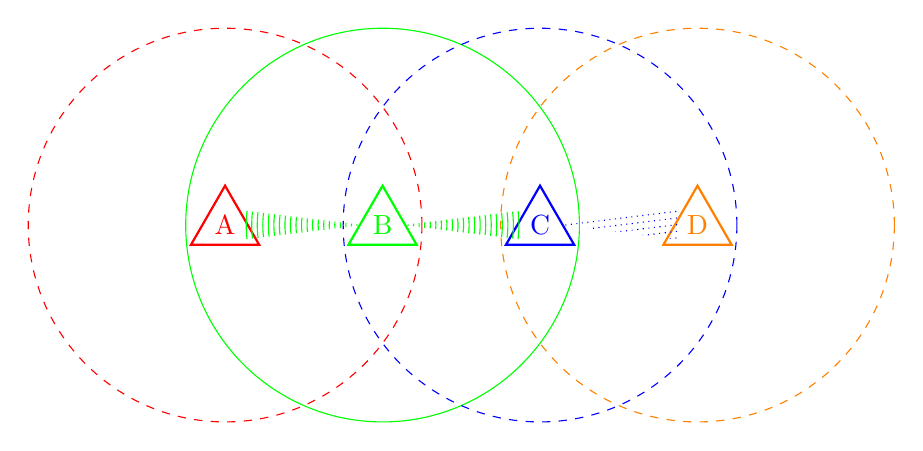
\begin{tikzpicture}
	% Signal radii.
	\draw[dashed, red] (-2, 0) circle [radius=2.5]; % A
	\draw[green] (0, 0) circle [radius=2.5]; % B
	\draw[dashed, blue] (2, 0) circle [radius=2.5]; % C
	\draw[dashed, orange] (4, 0) circle [radius=2.5]; % D

	% Base stations.
	\basestation{BS1}{A}{red, shift={(-2, 0)}};
	\basestation{BS2}{B}{green};
	\basestation{BS3}{C}{blue, shift={(2, 0)}};
	\basestation{BS4}{D}{orange, shift={(4, 0)}};

	% Signal arrows.
	\draw[green, transmission] (BS2) -- (BS1);
	\draw[green, transmission] (BS2) -- (BS3);
	\draw[blue, transmission, dotted] (BS3) -- (BS4);
\end{tikzpicture}
\end{center}
\end{document}